%!TeX TXS-program:bibliography = txs:///biber
%!TeX program = xelatex
\documentclass[research,19]{idcc}
\usepackage[utf8]{inputenc}
\usepackage{graphicx}
\usepackage{listings}
\usepackage{hyperref}
\hypersetup{
	colorlinks,
	linkcolor={black},
	citecolor={black},
	urlcolor={blue}
}
\usepackage{float}
\usepackage{acronym}
\usepackage{setspace}
\usepackage{csvsimple}
\usepackage{longtable}
\usepackage{xspace}

\acrodef{DOI}{Digital Object Identifier}
\acrodef{DC}{Dublin Core}
\acrodef{PSID}{Panel Study of Income Dynamics}
\acrodef{ICPSR}{Inter-university Consortium for Political and Social Research}
\acrodef{CMS}{Content Management System}
\acrodef{HCI}{Human-Computer Interaction }
\acrodef{DAS}{Data Accessibility Statement}
\acrodef{FAIR}{Findable, Accessible, Interoperable and Reusable}
\acrodef{FSRDC}{Federal Statistical Research Data Center}
\acrodef{FTI}{Federal Tax Information}
\acrodef{NSO}{National Statistical Organization}
\acrodef{LBD}{Longitudinal Business Database}
\acrodef{PID}{persistent identifier}
\acrodef{AEA}{American Economic Association}
\acrodef{API}{Application Programming Interface}
\acrodef{CSS}{Cascading Style Sheets}
\acrodef{URL}{uniform resource locator}
\acrodef{IDCC}{International Digital Curation Conference}
\acrodef{RDA}{Research Data Alliance}
%\usepackage{natbib}
%\usepackage[sorting=nyt,maxnames=10,backend=biber]{biblatex}
\usepackage[style=apa,sortcites,backend=biber,date=year]{biblatex}
\AtEveryBibitem{\clearfield{month}}
\AtEveryBibitem{\clearfield{day}}
%\DeclareLanguageMapping{american}{american-apa}
\DeclareLanguageMapping{british}{british-apa}
\addbibresource{references.bib}
\addbibresource{references-zotero.bib}
\addbibresource{aej-rep.bib}


% Table
\usepackage{array}
\newcolumntype{L}[1]{>{\raggedright\let\newline\\\arraybackslash\hspace{0pt}}p{#1}}
\newcolumntype{C}[1]{>{\centering\let\newline\\\arraybackslash\hspace{0pt}}p{#1}}
\newcolumntype{R}[1]{>{\raggedleft\let\newline\\\arraybackslash\hspace{0pt}}p{#1}}

% Different ways to cite URLS
%\newcommand{\urlcite}[2]{\href{#1}{#2}
\newcommand{\urlcite}[2]{#2\footnote{\url{#1}}}

\newcommand{\metajelo}{\texttt{metajelo}\xspace}

%
% Metadata
\author{Carl Lagoze}
\affil{University of Michigan}
\author{Lars Vilhuber}
\affil{Cornell University}
\correspondence{Lars Vilhuber. Email: \email{lars.vilhuber@cornell.edu}}
\title{metajelo: A metadata package for journals to support external linked objects}

%\conference{14th International Digital Curation Conference}
\submitted{June 2018}



\begin{document}
\maketitle

\begin{abstract}
	We propose a metadata package that is intended to provide academic journals with a lightweight means of registering, at the time of publication, the existence and disposition of supplementary materials.  Information about the supplementary materials is, in most cases, critical for the reproducibility and replicability of scholarly results.  In many instances, these materials are curated by a third party, which may or may not follow developing standards for the identification and description of those materials.  As such, the vocabulary described here complements existing initiatives that specify vocabularies to describe the supplementary materials or the repositories and archives in which they have been deposited.  Where possible, it reuses elements of relevant other vocabularies, facilitating coexistence with them.  Furthermore, it provides an ``at publication'' record of reproducibility characteristics of a particular article that has been selected for publication.  The proposed metadata package documents the key characteristics that journals care about in the case of supplementary materials that are held by third parties: existence, accessibility, and permanence. It does so in a robust, time-invariant fashion at the time of publication, when the editorial decisions are made. It also allows for better documentation of less accessible (non-public data), by treating it symmetrically from the point of view of the journal, therefore increasing the transparency of what up until now has been very opaque.
\end{abstract}

\section{Introduction}
\label{sec:intro}
Reproducibility and replicability of scientific findings has been given greater scrutiny in recent years (REFS). Scientific journals, whether run by publishing companies (Springer, Elsevier, etc.) or learned societies (American Economic Association, Midwest Political Science Association, American Statistical Association, Royal Statistical Society, to name just a few in the social and statistical sciences), have been playing an important role in supporting these efforts for many years, and continue to explore novel and better ways of doing so. In particular, several journals have been hosting ``supplementary materials'' on their own journal websites or on affiliated repositories (e.g., Harvard Dataverse, Figshare) in support of reproducibility of the work described in published scientific articles. Data and code deposits are requested after authors' work has been (conditionally) accepted after peer review, or, less frequently, as part of the original manuscript submission process. In doing so, they assume for themselves (or delegate to a single trusted third party) the curation role for these materials, and can therefore know with certainty how long and how accessible these materials are to be preserved.

Authors are increasingly being encouraged and trained in reproducible methods from the outset of their research projects, rather than performing ex-post documentation. This includes carefully documenting provenance of third-party datasets being used, and properly curating generated datasets (surveys, collected data, etc.) in data archives as soon as possible. Furthermore, in at least some social sciences, the use of pre-existing but non-public data has increased substantially.  Confidentiality and licensing constraints prevent authors from depositing such data in open archives. Journals must rely on an increasingly diverse cadre of data-holding institutions, not all of which are ``archives'' in the traditional sense, while satisfying increasing scrutiny of the provenance of the research results published by them. Both scenarios - early and third-party deposit of data and use of restricted-access data - make it difficult for journals and traditional archives to carry out their curation role. The resulting lack of transparency in data provenance is detrimental to the overall effort of increasing transparency in the sciences.

The approach outlined in this article proposes a metadata package, derived from existing metadata schemata where possible, that provides a lightweight approach to ameliorating this problem. In particular, the proposed metadata package documents the key characteristics that journals care about in the case of supplementary materials that are held by third parties: existence, accessibility, and permanence. Our intent in defining the metadata package is two-fold. First, the package enables  authors to provide the information as they submit articles to journals, allowing informed editorial decisions to be made. Second, at the time of publication, the information is made public, providing robust documentation on data provenance in an immutable package, in a compact fashion.  The package allows for better documentation of any data, regardless of the difficulty of access.   Thus the information provided for less accessible (non-public data) is improved by treating it symmetrically with open access data, therefore increasing the transparency of what up until now has been very opaque.

We start by providing a detailed use case. We relate our approach to existing metadata, both in terms of structure as of content, and then describe the metadata package. We conclude by discussing some usability issues for three contributors or consumers of this information, and an outlook on a possible implementation.

\section{Background}
\label{sec:background}
In most applied sciences,
it has become common publication practice to provide evidence of the
statistical or laboratory data underlying the conclusions. This is done
to support reproducibility and replicability of the scientific
findings.%
\footnote{There is considerable heterogeneity in the use of the terms
	``reproducibility'' and ``replicability''. In this paper, we will adopt
	the following definitions: reproducibility is ``the ability of a
	researcher to duplicate the results of a prior study using the same
	materials and procedures as were used by the original investigator,''
	\parencite{BollenSocialBehavioralEconomic2015} whereas replicability
	differs in that ``new data are collected.'' (ibidem).} 
Journals with a
data deposit policy have stored the supplementary materials on journal
websites, often as simple web-based ZIP archives. While ensuring that
the materials are preserved as long as the journal is active
(\textit{permanence}) and are accessible to any reader of the original article (\textit{accessibility}), certain shortcomings became
apparent. Very large datasets and datasets with confidentiality concerns
were nearly always out of scope. 

More recently, journals have leveraged
either dedicated, journal-branded views onto larger archives (e.g,
Dataverse, Figshare), built their own data archive infrastructure
(\urlcite{https://www.elsevier.com/authors/author-services/research-data}{Elsevier/Mendeley}), or have allowed for data and code to be stored
more generally on any of a curated list of ``trusted'' or ``approved''
whitelist of third-party repositories.%
\footnote{\url{https://f1000research.com/for-authors/data-guidelines}, \url{https://www.nature.com/sdata/policies/repositories}}
Each of these alternatives rely
on a journal or publisher ``vetting'' the repositories and ascertaining
that it meets some set of criteria.  While some third-party vetting of
repositories exists,%
\footnote{CoreTrustSeal, \url{https://www.coretrustseal.org/}}
it is far from being universally accepted at this
time. 

In all cases known to us, the support for restricted-access
repositories is quite limited. Thus, most of the known support for
third-party repositories does not provide much information about
accessibility (the presumption is that access is open), nor about the
permanence of the repositories - this is presumably one of the
evaluation criteria that journals and publishers use, but is not clearly
defined as such. In fact, at least one of the consulted publishers
explicitly allows for quite transitory repositories for code, without
clearly distinguishing that from archives that are more permanent.%
\footnote{F1000Research (\url{https://f1000research.com/for-authors/data-guidelines}) allows for code deposits through github.com, which has no mandate to preserve, and allows code owners to delete materials at any time without restrictions.}

Nevertheless, much of the information about persistence of archives and
materials stored within those archives is available, albeit in
idiosyncratic and non-machine readable form. Consider only the case of
national archives (e.g., the \urlcite{https://www.archives.gov/dc/researcher-info}{U.S. National Archives} or the \urlcite{http://www.archives-nationales.culture.gouv.fr/}{\textit{Archives Nationales} in France}). 
In general, data stored in national archives is
permanently archived; if it is not, this is clearly documented.%
\footnote{For instance, the program code for the Business Register is destroyed when a new system is put in place - they are never kept \parencite{U.S.CensusBureauRecordsControlSchedule2009}. Unedited master files for the American Community Survey are destroyed 6 years after the Edited master files are verified, unless still needed ``for Census operations'' \parencite{U.S.CensusBureauRecordsControlSchedule1999}.}
Furthermore, access is generally not restricted - if it is, this is
clearly documented. However, materials in national archives do have
certain restrictions - they may require sending in a written request, or
a physical visit to a location with copies of the data. Thus, while the
information may satisfy the publication requirements of even the most
open journal, there is no robust and standardized way of documenting the
additional restrictions on access that persist. 

In proposing the
metadata package outlined in this article, we attempt to improve on this
situation. By providing a sparse but sufficient encapsulation of the
information collected from authors, archives, and other third-parties,
we create greater transparency about the data supporting the research.
By relying on existing metadata schemas and metadata content, we
minimize the effort by all parties involved, increasing the likelihood
of adoption. And by intrinsically addressing the possibility that the
information obtained at the time of publication may differ from that returned by later
requests for the same information, we provide the tools to journals,
publishers, and their editors to document that the decision to publish
was based on adequate information at the time of the publication (or
acceptance decision).



\section{Use Case}
\label{sec:usecase}
We target a specific but very common use case. A researcher has written a paper with empirical content, and is required by the journal's data and code availability policy to prepare a ``replication package.'' The journal's policy requires that the code and data be accessible to others, but does not require deposit of the materials as a ``supplementary file,'' i.e., as a ZIP file on their website.\footnote{In fact, some journals may not offer that option.} However, in all cases, the journal wishes to ascertain three key attributes of the replication package or packages:
\begin{itemize}
    \item the \textit{existence} of the package
    \item the \textit{access rules} to the package (license, terms of use)
    \item the \textit{persistence} of the package
\end{itemize}
In an ideal scenario, the existence of the package can be easily ascertained in a reputable repository, it is made available under an well-specified (ideally open) license, and it is available ``forever''. When the journal manages its own repository, these attributes are known. When the package is available elsewhere, these attributes need to be discovered. Furthermore,  this needs to happen in a scalable,  automated, and reusable fashion, as it should be feasible to do so for all articles, submitted to any journal. 

\subsection{Current Metadata Infrastructure and Use Cases}
The current metadata infrastructure should be expected to work well for open-access data deposits. Deposits are encouraged in known repositories such as \ac{ICPSR}, Zenodo, or the \urlcite{https://osf.io}{Open Science Framework}, which have been vetted according to certain criteria by the journals themselves.

But what if an author has deposited the information in a reputable but unlisted repository, for instance the \urlcite{https://ada.edu.au/}{Australian Data Archive}? Emails are to be exchanged, and some case-by-case vetting of repositories, their reliability, and whether they assign \ac{DOI} is performed. FAIRsharing.org and re3data are invoked to ascertain their policies. 

In the Appendix, we demonstrate for three cases that this infrastructure - DataCite, re3data, and FAIRsharing - will fail on even simple scenarios. In all cases, we attempt to ascertain \textit{existence}, \textit{access rules} (terms of use and licenses), and \textit{persistence} (preservation policies) via machine-readable metadata. We fail to collect complete information in  all cases. Furthermore, as of the writing of this article, and presumably for some time yet, this infrastructure simply cannot support scenarios that use broadly available restricted-access data. By ``broadly available restricted-access'', we mean that a non-trivial fraction of a research community can be granted access to these data, which are restricted-access only for reasons of confidentiality. This scenario is quite common - it applies to clinical data in psychology as much as demographic data collected by national statistical agencies in every country in the world. 

The three cases are as follows. First, we show that a user-initiated data deposit of a digital  object at  \urlcite{https://www.openicpsr.org}{openICPSR}, properly recorded in DataCite, can at best reveal \textit{existence}, but cannot reveal the remaining attributes (\textit{access rules} and \textit{persistence}) through queries to the infrastructure. A customized parser can ascertain the \textit{license} by querying the landing page of the object. Queries to DataCite fail to elicit the  license because it is optional. Queries to re3data fail because a record cannot be found using information available through the \ac{DOI}, in particular, the name of the repository. Cheating somewhat, when we force a query to re3data's entry for \ac{ICPSR} \parencite{Re3data-icpsr}, it fails to yield correct information, presumably because the record is not maintained by ICPSR staff, and does not hold information on openICPSR policies. We fail to ascertain the preservation policy through queries to all sources, and only subject-matter expertise can find the information on ICPSR's website. 

The second query is for the \ac{PSID} Geospatial Data \parencite{psid-geodata}. The \ac{PSID} is a longitudinal household survey conducted by the University of Michigan, which began in 1968. More than 4000 peer-reviewed publications have used the data \parencite{psid-homepage}. The data are available without cost to researchers - but they do require that terms of use be agreed to before downloading, through registration. This is accurately reflected in the r3data entry for the \ac{PSID} \parencite{Re3data-psid}. However, we are considering the Geospatial Data, which is restricted data. re3data fails to record any information for this access mechanism. Furthermore, although \ac{PSID} has acted as a data curator for its own data for 50 years, it does not assign a \ac{PID} to the data. DataCite has no information on any  \ac{PSID} data holdings, which are only available through the \ac{PSID} website. Until recently, both non-restricted and restricted data could not be deposited at journal websites or other repositories, as per the terms of use.\footnote{This has changed recently with the introduction of an openICPSR-hosted \ac{PSID} repository, but see the issues above.} Finally, although the \ac{PSID} has, of course, a 50-year track record, no statement can be found on the website attesting for preservation plans, or for versioning of data (preservation of prior versions).\footnote{Personal communication in November 2018 with David S. Johnson, at the time Director of the \ac{PSID}, indicates that all versions of non-restricted and restricted data are preserved in a dark archive.}

The third example is a confidential dataset made available by a \ac{NSO}, in this case the U.S. Census Bureau, although it is typical of microdata holdings by \ac{NSO} around the world. The \ac{LBD} \parencite{LBD,MirandaJarmin2002} is one of the most widely used microdata files in the \ac{FSRDC} system. The \ac{FSRDC} system is used by nearly 700 researchers at 29 locations around the United States \parencite{u.s._census_bureau_center_2018}. As with the \ac{PSID}, entries for the U.S. Census Bureau exist on re3data \parencite{Re3data-uscb}, but have no information on the \ac{FSRDC}. No \ac{PID} have yet been assigned to any datasets. Furthermore, no data can be removed from the \ac{FSRDC}. Researchers must thus rely on the U.S. Census Bureau for preservation. In addition to the \ac{LBD} itself, which is presumably covered by a record schedule, detailing its preservation period, researchers also need to consider the preservation of any derivative files they wish to make available as part of their research. If these are aggregated results (model coefficients, etc.), they are released by the U.S. Census Bureau to the researcher. Microdata cannot be released. Most of this information is provided to researchers when they obtain access, but cannot easily be communicated to journal editors or readers of articles. Nevertheless, as we have argued  
\iftoggle{blind}{[BLINDED]}{\parencite{Lagoze2017-qv}} and experienced in our own research 
\iftoggle{blind}{[BLINDED]}{\parencite{AbowdVilhuber2005,AbowdEtAl2009c,McKinneyEtAl:submitted:2017}}, it is definitely feasible to do reproducible research in this environment. The difficulty consists in communicating that information, in a reliable fashion, to editors, referees, and readers.




\subsection{Common Denominator}
We have chosen three types of datasets -- public-use, restricted-access with light restrictions, restricted-access with strong restrictions --, curated by three different institutions -- an open repository, a panel survey  provided by a recognized leader in the field, and confidential business microdata provided by one of the largest and oldest \ac{NSO} in the world -- all with impeccable data curation reputations. The choice is idiosyncratic, but it presumably is symptomatic of the still young state of the metadata infrastructure. We don't believe these examples are exceptions - similar institutions exist all over the world, and we could as easily have done such examples with data from Australia \parencite{PTKLYP_2018}, Germany (Research Data Centre (FDZ) of the German Federal Employment Agency (BA) at the Institute for Employment Research (IAB)). Presumably, counterexamples can be given. But journal editors and authors need such mechanisms to be broadly feasible if they are to use them. At present, that is not the case.

We set out to accomplish this by designing a  metadata package, drawing on existing schema used within the infrastructure, but populating it in a decentralized fashion, at the point of first use: the journal submission system, or if the researcher uses a reproducible workflow, at data acquisition by the researcher. An associated application can leverage the metadata infrastructure where it does provide information,  and pre-fill any fields. However, when ambiguous responses are obtained, or no information is available, the researcher can provide guided or verbatim answers. At both points in time, the researcher has the best incentives to provide the information accurately -- the acceptance of the submission may depend on the accuracy of the information -- and the most timely recollection of where to obtain the information.



\section{Related Metadata and Efforts}
\label{sec:related-metadata}
A number of other initiatives address the issue of reusability and replicability, some of them through proposed metadata standards.  We have endeavoured to leverage these efforts when possible (i.e., when semantics of tags overlap with our goals and when their XML schema are designed for reuse).  Our hope is that this makes both interoperability with those efforts as easy and possible, and that the use of already established and perhaps familiar tags and attributes decreases the learning curve for use of our proposed schema.  In the remainder of this section we describe related initiatives and the influence they have on our metadata design.

\subsection{DataCite}
The most related metadata vocabulary comes from \urlcite{https://www.datacite.org/}{DataCite}, which provides infrastructure to locate, identify, and cite research data. Identification is done via the DOI infrastructure for persistent identification, which has emerged as the standard for naming scholarly objects.  The DataCite metadata schema \parencite{DataCiteMetadataWorkingGroupDataCiteMetadataSchema2017a,DataCiteMetadataWorkingGroupDataCiteMetadataSchema2017} specifies elements and attributes to describe data resources for the purpose of citation, location and retrieval.  Because of the notable overlap in the purpose of DataCite  and our proposal, we make use of multiple parts of this schema. Note, however, that DataCite is targeted as describing the data products themselves, where our concern is to register the placement of those products in a repository and ancillary information about that placement.

\subsection{Re3data}
The goal of describing repositories and archives for data curation is directly addressed by the Re3data initiative \parencite{RucknagelMetadataSchemaDescription2015,Re3data.Orgre3dataorgMetadata2015}.  The goal of Re3Data is to support an online registry of research data repositories.   The mechanics underlying this is to establish a common metadata standard for describing such repositories, This metadata is then used to power a search interface.  The registry and search interface are targeted at researchers searching for the appropriate repository in which to store their data.
A primary technical output of the work of re3data is a ``Metadata Schema for Description of Research Data Repositories'' now in its 3rd version and expressed as an XML schema.  The schema addresses repository characteristics such as identification,   language, administrative contacts, subject focus, funding basis and the like.  Our work addresses repository characteristics and reuses semantics from the Re3data schema where appropriate and possible.  We will describe the details of this reuse later in this paper.

\subsection{CrossRef}
\urlcite{https://www.crossref.org/}{CrossRef}  sits functionally between our work and the two initiatives described above.  It was conceived by publishers as a DOI registry that, in addition to providing the resolution of those DOIs, stores metadata for the corresponding scholarly object.  An important aspect of this metadata are cross-references (citations) among the named objects \parencite{CrossRefRelationshipsDOIsother}.  In that sense, CrossRef acts as a ``switchboard'', documenting linkages between scholarly objects. Originally, the linkages were citations between journals, but with increasing interest in data these linkages have been expanded to include these supplementary materials.  In this context, CrossRef collaborates and interoperates with DataCite, with the former focusing on registration and description of journal articles and conference papers, and the latter on data and other supplementary artifacts .  The CrossRef schema is a relatively complex tag set for describing articles.  As our intention is to promote a lightweight approach (not necessarily exclusive but perhaps in tandem with CrossRef), we have not directly borrowed from their schema.  Also, our focus is linking to repositories or archives that contain supplementary material, as opposed to the object itself.

\subsection{Scholix}
The Scholix effort \parencite{BurtonScholixMetadataSchema2017} is also closely related to our proposed package. However, while it may lay the groundwork for the information here, it fundamentally does not have rich enough information about the linked objects to fulfill our core purpose.

\subsection{CoreTrustSeal}
Two additional related initiatives are worthy of mention.   The Core Trustworthy Data Repository Requirements \parencite{CoreTrustSealDataRepositoriesRequirements2017} are the result of work within the Research Data Alliance to establish standards for so-called ``trustworthy'' repositories.  These are repositories that meet a set of criteria that deem them dependable for the long-term curation of data.  The criteria are a mixture of technical, administrative, financial, and personnel characteristics.  The criteria are not as of yet, or planned to be, encoded in a machine-readable schema.  Instead, repositories apply for trusted status through a form that his reviewed by a human board of review.  Our proposed metadata format allows for the attribution of a repository as ``trusted'' and thus integrates minimally with the CoreTrustSeal effort.

\subsection{JATS}
The \urlcite{https://jats.nlm.nih.gov/}{JATS (Journal Article Tag Suite)}, led by the NCBI (National Center for Biotechnology Information) aims to develop specifications for standardized (XML) markup for scholarly articles.  The effort grows out of work done on so-called ``NLM DTDS'', which modelled tag sets for scholarly document structuring.  \urlcite{https://jats4r.org/}{JATS4R} (JATS for reuse) is a follow-on effort, designed to reuse and extend XML models defined by JATS, with the primary goal of facilitating reuse of existing scholarly material (publications and supplementary data). The result is a set of models specifying document structure, rather than simply metadata.  The structural elements address issues such as how to mark-up authors and affiliations, citations, data citations and the like.

\subsection{Data Accessibility Statements}
The Belmont Forum has recently started \urlcite{a project}{http://www.bfe-inf.org/resource/belmont-forum-data-publishing-policy-workshop-report-draft} to standardize a \ac{DAS}. Its goals seem to be quite similar to our project, and while independently developed, we look forward to seeing their suggestions, and will collaborate in moving that forward.

\section{Metadata Package}
\label{sec:metadata-package}
\label{sec:approach}
The high-level structure of our proposed metadata package is illustrated in the Figure~\ref{fig:schema_v1} (produced by OxygenXML). 
\begin{figure}
	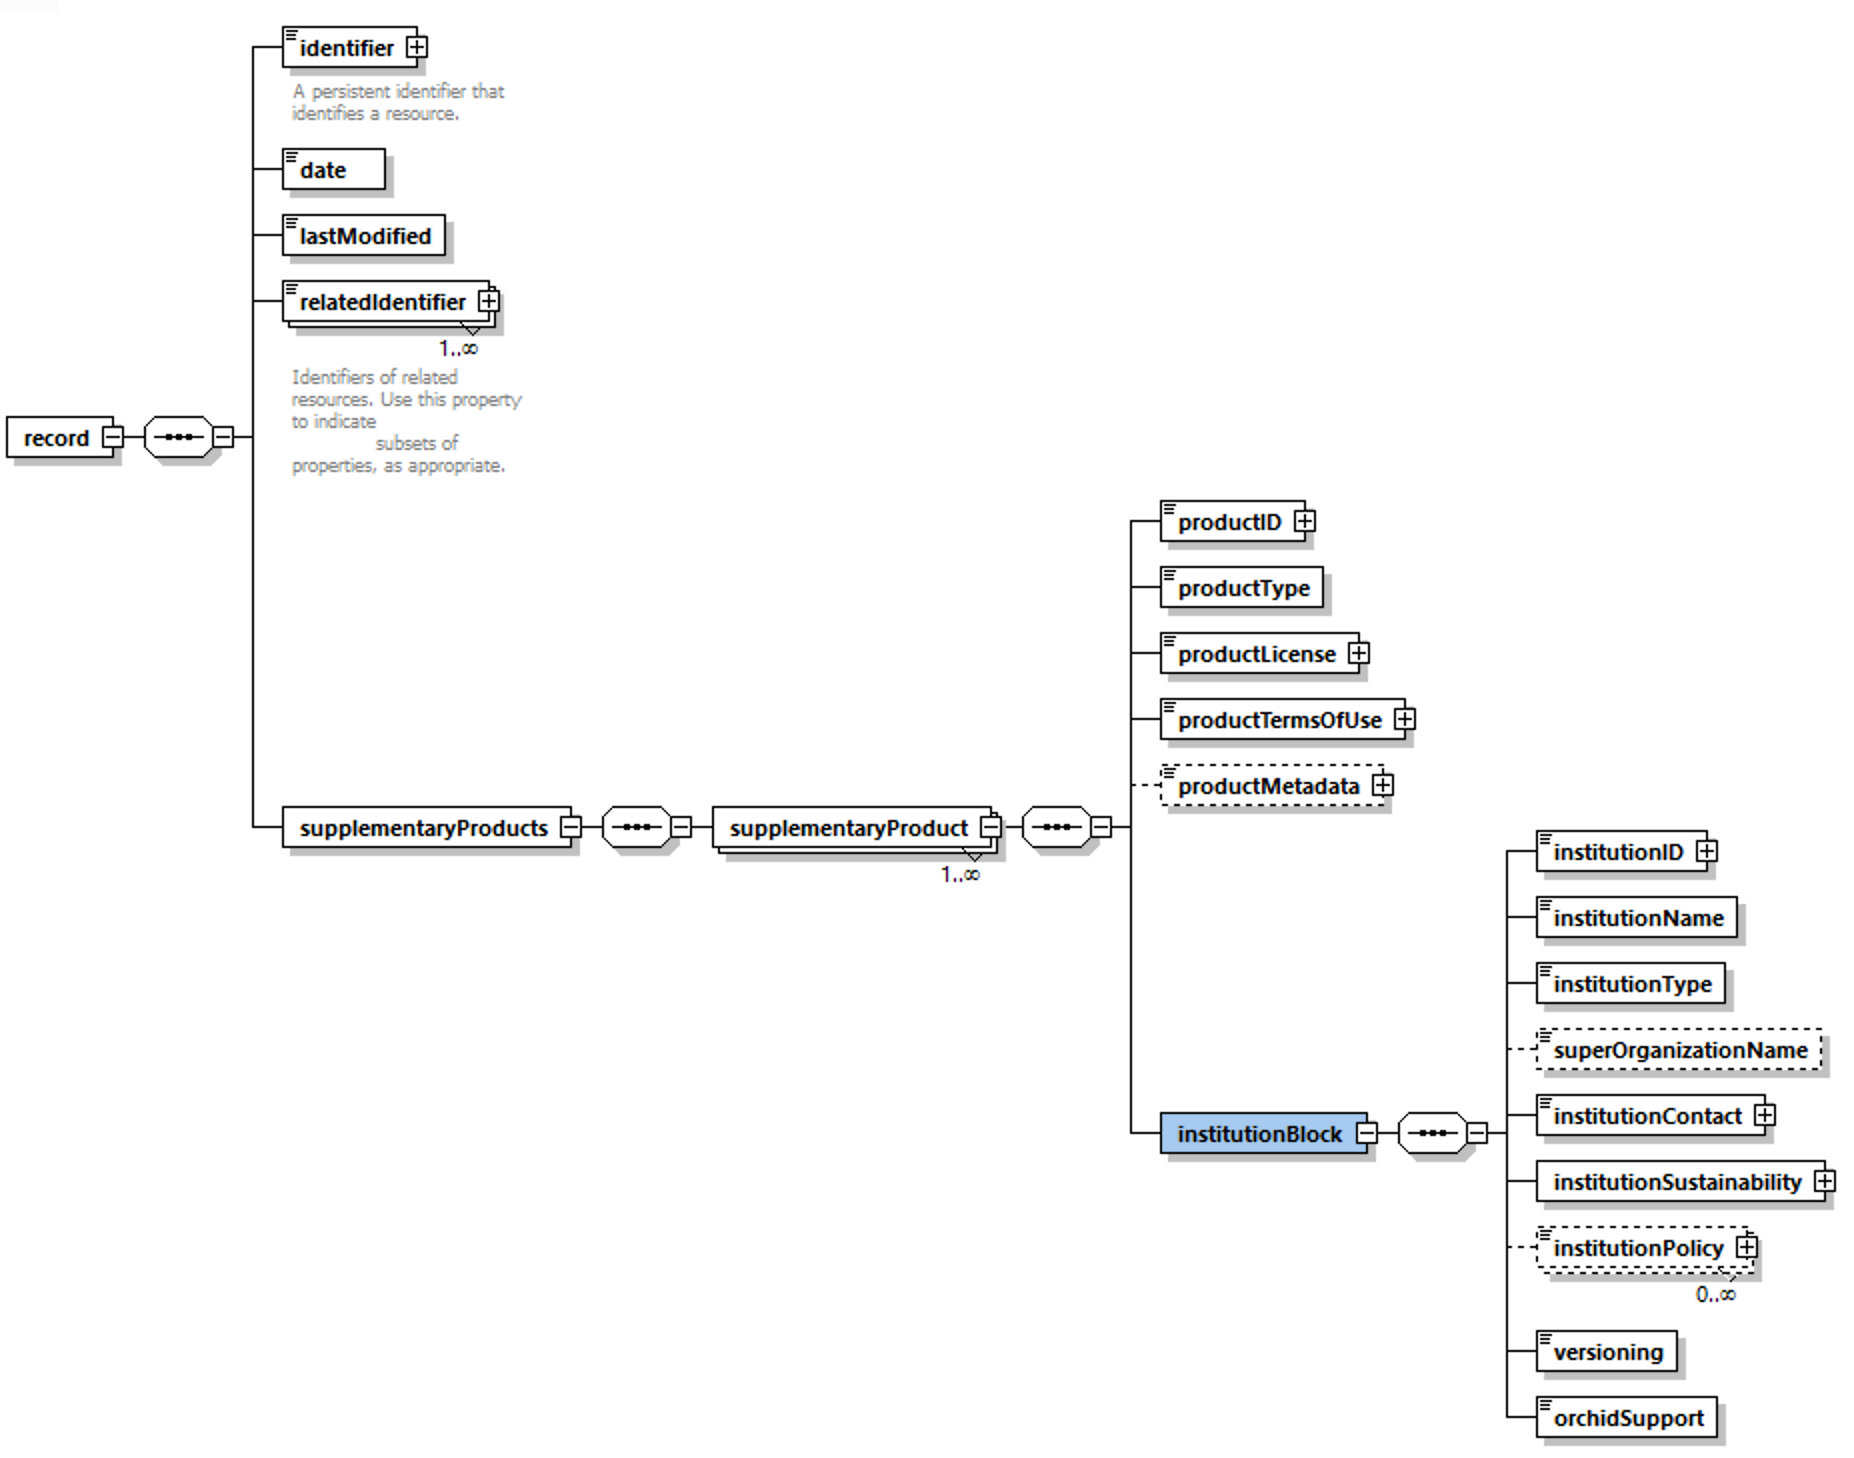
\includegraphics[width=\textwidth]{images/schema_v1}
	\caption{\label{fig:schema_v1}High-level structure of proposed package}
\end{figure} 
As shown, each package is structured as a record, which conceptually models a linkage between a publication and its supplementary materials.  As shown, a record has an identity (\ac{DOI}), a date created, a last modified date, and the identity (\ac{DOI}) of the research objects (papers) that are associated with the supplementary products.
Each record then can describe an unlimited number of \texttt{supplementaryProducts}.  Each product has an identifier, a description of its type, licensing information, and linkages to full metadata available elsewhere that fully describes the product.  Each \texttt{supplementaryProduct} has an associated location block, which contains information about the institutional archive at which the respective \texttt{supplementaryProduct} is located.  Finally, for each institution, the set of possible policies are listed, with a boolean designation of the applicability of a policy to the respective supplementary object.   
The full annotated schema is available for examination online at \href{https://github.com/labordynamicsinstitute/metajelo}{github.com/labordynamicsinstitute/metajelo}.

%id;field;description;comment;source;larscomment
\csvreader[/csv/separator=semicolon,/csv/head=true,%
/csv/before reading=\footnotesize%
\setlength{\tabcolsep}{2.5pt},%
/csv/after reading=\normalsize,%
/csv/head to column names=true,%
/csv/longtable=L{0.1\textwidth}L{0.25\textwidth}L{0.3\textwidth}L{0.2\textwidth}L{0.1\textwidth},
/csv/table head=%
 \multicolumn{5}{c}{Table~\thetable : \metajelo Description\label{tab:desc:metajelo}}\\%
 \hline \bf ID & \bf Field &\bf Definition & \bf Notes &\\\hline\endfirsthead%
 \multicolumn{5}{c}{Table~\ref{tab:desc:metajelo} : \metajelo Description}\\%
 \hline \bf ID & \bf Field &\bf Definition & \bf Notes &\\\hline\endhead%
  \hline\endlastfoot%
 \hline&&&\multicolumn{2}{r}{(cont)}\\\endfoot,
/csv/late after line=\\\hline,
table foot=\hline%
]%
{../schema/tabular-metajelo.csv}{}{%
	\id &\field &\description &  \comment & \source 
}



\section{Usability Notes}
\label{sec:usability}
Academic publishing outsources much of the content-related work to authors and subject matter editors. In order to be useful, the proposed package needs tools around it. We sketch out two such tools, and also address the role archives and repositories themselves play. 
\subsection{Metadata ingest}

We envision that the package be provided as a single file during the manuscript submission process by the author. This ensures that existing editorial workflow packages can seamlessly track the package, without needing upgrades to understand the content. The package can be inspected by curation specialists and data editors and made available to reviewers as needed, and will follow the main document throughout the review process. 
           
\subsection{Creation by authors}
In order to create the package, we envision a simple website, which helps authors fill in the required information. Appropriate \ac{HCI} testing would need to be done to determine the optimal structure. However, the starting point is the DOI of the object being described. From the DOI, a backend query to DataCite or CrossRef can reveal the hosting institution's institutionID. In turn, lookup in re3data or fairsharing.org will reveal elements of the institutional policies with regards to general access or preservation. Institutions often have multiple access policies and licenses, and which one applies to the object identified by the DOI may be hard to determine automatically. The author will be able to choose the appropriate license she consented to from a set of choices appropriate for the object and its hosting institution. In theory, all such information is provided through re3data, but failing to look up complete or accurate information, the author can also fill in the information manually. 
           
\subsection{Hosting by journals}
Journals are expected to post the package on their website, on the same landing page as the article itself. By doing so, the package itself can be parsed by appropriate in-page Javascript (provided through a open source library), and displayed with appropriate CSS (also provided through an open source library). Naturally, more complex journal websites can include the contents in the page source code or in their \ac{CMS}. 

\section{Acknowledgements}
\label{sec:ack}
Lagoze and Vilhuber acknowledge funding received from \href{http://www.nsf.gov/awardsearch/showAward.do?AwardNumber=1131848}{NSF Grant \#1131848} (NCRN) and the American Economic Association. The views and recommendations expressed herein are those of the authors, and not those of either the American Economic Association or the National Science Foundation.


%\bibliographystyle{chicagoa}
%\bibliography{references.bib}
\printbibliography


%\appendix

\section{Appendix: Detailed Use Cases}
\label{app:cases}

\newcommand{\suppDir}{supplementary_materials}
In all use cases, we attempt to identify the three attributes outlined in the main text, using automated mechanisms.

\section{Use Case 1: Public-use information at openICPSR}
In the first case, the researcher has  used public-use data, and identifies a \ac{DOI} to the journal (\url{http://doi.org/10.3886/E100590V1}).  We thus start with the \ac{DOI}, which resolves to the following citation:

\lstset{numbers=left,numberstyle=\tiny,stepnumber=1,basicstyle=\linespread{0.8}\footnotesize}
\begin{quote}
	\it
	McKinney, Kevin L., Green, Andrew S., Vilhuber, Lars, and Abowd, John M. Replication data: Total Error and Variability Measures for QWI and LODES. Ann Arbor, MI: Inter-university Consortium for Political and Social Research [distributor], 2017-12-15. https://doi.org/10.3886/E100590V1
\end{quote}

%We note that this dataset, as all current openICPSR datasets, is licensed under a \href{http://creativecommons.org/licenses/by/4.0/}{Creative Commons Attribution 4.0 International License}. 
\FloatBarrier
\paragraph{DataCite}

We first query the DataCite API (Figure~\ref{fig:case1:datacite}).
\begin{figure}
	\singlespacing
	\lstinputlisting[language=xml,linerange=1-1]{\suppDir/datacite-api-100590.xml}
	\lstinputlisting[language=xml,linerange=9-9,firstnumber=9]{\suppDir/datacite-api-100590.xml}
	\lstinputlisting[language=xml,linerange=10-10,firstnumber=10,basicstyle=\bfseries\footnotesize]{\suppDir/datacite-api-100590.xml}
	\lstinputlisting[language=xml,linerange=11-11,firstnumber=11]{\suppDir/datacite-api-100590.xml}
	\lstinputlisting[language=xml,linerange=22-22,firstnumber=22]{\suppDir/datacite-api-100590.xml}
	\lstinputlisting[language=xml,linerange=23-24,firstnumber=23,basicstyle=\bfseries\footnotesize]{\suppDir/datacite-api-100590.xml}
	\caption{Select lines from DataCite query for DOI 10.3886/E100590V1}
	\label{fig:case1:datacite}
	\centering \footnotesize The full query response can be found in the appendix.
\end{figure}
%
The query reveals the identity of the \texttt{datacentre} and the \texttt{publisher}. However, there is no information on the license under which the object is made available, no copyright, license, or terms of use information, nor any information on persistence of the data. The \texttt{license} attribute is optional as per DataCite Schema \parencite{DataCiteMetadataWorkingGroupDataCiteMetadataSchema2017}, and is empty here.

\paragraph{re3data}
We turn to re3data for further information, and find two possible problems. A lookup for the contents of the \texttt{datacentre} field yields 0 results. A search for the contents of the \texttt{publisher} field yields a wrong result (\lstinline|<odesi>|). We applied human judgment to find a re3data record for ICPSR: \url{https://www.re3data.org/repository/r3d100010255} \parencite{Re3data-icpsr}. We note, however, that the rules and policies for openICPSR may differ from \urlcite{https://www.openicpsr.org/openicpsr/faqs}{ICPSR}.
The re3data record lists three types of data access. Furthermore, three data licenses are listed: two \texttt{other} and one \texttt{copyright}.
\begin{figure}[H]
	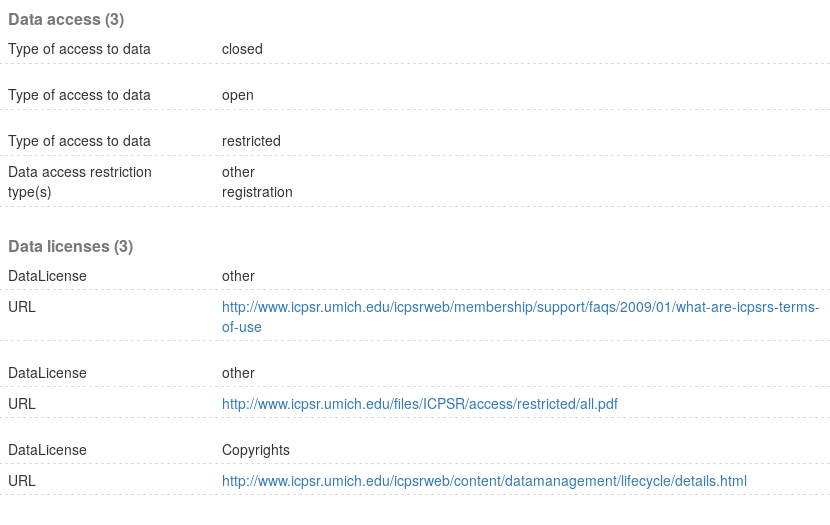
\includegraphics[width=1\textwidth]{\suppDir/re3data-org-icpsr-access-licenses-20181008.png}
	%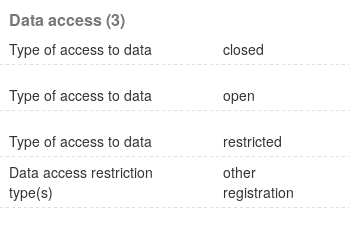
\includegraphics[width=0.4\textwidth]{re3data-org-icpsr-access-20181008.png}
\end{figure}
Thus, while re3data does contain entries of \textit{possible} licenses, we have no information on which one applies to the replication package above. Furthermore (not displayed here), there is no machine-readable information on persistence. While knowledgable data archivists and librarians, as well as many social scientists, ``know'' that ICPSR is a reputable archive with a long history and presumably a long future, this is not encoded anywhere where non-domain experts could ascertain it.

\paragraph{CoreTrustSeal}
We do not investigate whether this information is available  through CoreTrustSeal, for three reasons. First, searching again, as we did, through the website, neither of the search terms that the DataCite record provides yield findable results. Second, when we manually identify ICPSR on the website's map of institutions, we observe that ICPSR had a ``Data Seal of Approval'' (the predecessor to CoreTrustSeal), but that it expired in 2017, which may explain the lack of search results. Finally, the CoreTrustSeal certification is encapsulated in PDFs, and does not provide an API to search for attributes of a certified repository. While it may be feasible for a human to track down the relevant information, it is not scalable.
\FloatBarrier
\paragraph{Data publisher website}
\newcommand{\icpsrdate}{8 October 2018}
\begin{figure}
	\lstinputlisting[language=xml]{\suppDir/extract-webpage-20181008.xml}
	\caption{Use Case 1, Encoding of license in HTML of landing page}
	\label{fig:case1:rela}
\end{figure}
\begin{figure}
	\centering
	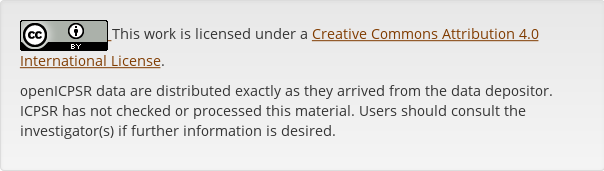
\includegraphics[width=0.5\linewidth]{\suppDir/../images/openicpsr-license-image.png}
	\caption{Use Case 1, license as displayed on website on \icpsrdate }
	\label{fig:case1:license}
\end{figure}
Finally, we attempt to obtain metadata   directly from the landing page indicated by the \ac{DOI}.%
\footnote{The query was run on \icpsrdate .}
The page offers five types of metadata: the in-page metadata in XML format, in-page metadata encoded as JSON-LD, a link to a OAI-PMH record, a link to a DDI 2.5 record, and a link to a DDI 3.1 record.
The webpage provides two instances of license information. The first instance is within the \texttt{rel} identifier within the \lstinline|a| link field (Figure~\ref{fig:case1:rela}) with an associated displayed  license badge (Figure~\ref{fig:case1:license}).
The second instance is encoded in the JSON-LD payload,
\begin{lstlisting}
"license":"https://creativecommons.org/licenses/by/4.0/deed.en_US"
\end{lstlisting}
Both provide the same information about the license.


\paragraph{Conclusion on Use Case 1}
We note that re3data did not provide additional information about  accessibility, even though ICPSR does provide data with more restrictive access rules, for instance, through secure cloud instances. Furthermore, no information is provided  about persistence. The openICPSR FAQ contain such information, but do so somewhat obliquely, and do not point to a policy. Browsing the website, one might encounter the ``\href{https://www.icpsr.umich.edu/icpsrweb/content/datamanagement/preservation/policies/index.html}{Digital Preservation Policies and Planning at ICPSR}'' \parencite{icpsr-preservation}, which  lays out the policies. 

We note that DataCite, while providing a means to communicate the license, did not do so at this time. DataCite does not provide a means to convey access rules or persistence, nor does it provide a means to point to specific policies on re3data. Re3data, in turn, lists three possible licenses, none of which apply in the present case, possibly because it lists information on the main ICPSR repository, and not on the associated but distinct openICPSR instance.

In this relatively straightforward case, we would need to query the user  about  which access policy applies to the particular dataset at hand. 

\section{Use Case 2: Restricted-access PSID}
The \ac{PSID} has published data for several decades, and is widely used (several thousand articles). Currently, researchers access the data by downloading them from the \ac{PSID} website, if the data is public-use. \ac{PSID} also provides some restricted access files, for instance with more detailed geocodes. Access procedures are described at \url{https://simba.isr.umich.edu/restricted/ProcessReq.aspx}. The \ac{PSID} has not assigned \ac{DOI} to any of its data products. Personal communication reveals that both public-use and restricted-access data are versioned internally, and that the data themselves contain a variable with the versioning information; there is, however, no metadata on the website listing the available past datasets, only the most current one. There is no explicit retention information on the website.

In this scenario, 
\begin{itemize}
	\item CrossRef or DataCite offer no information on the data
	\item While there is a re3data page at \url{https://www.re3data.org/repository/r3d100011131} \parencite{Re3data-psid}, it does not provide information on the restricted access conditions
	\item the product page offers some unstructured information
\end{itemize}
We also note that even if re3data had the correct access policy for 2018, it is difficult to obtain information on past access policies. The \ac{PSID} used to provide restricted-access data via shipment of CDs to researchers, who would put the data on computers that were not connected to networks, secured in a locked room. Authors are still publishing articles today that rely on data obtained through the outdated access mode. 

\section{Use Case 3: Restricted access at the U.S. Census Bureau}

The \ac{LBD} data \parencite{MirandaJarmin2002,LBD}  at the U.S. Census Bureau is one of the most requested datasets in the \ac{FSRDC} network. Access procedures are described at various locations, including \urlcite{https://www.census.gov/ces/rdcresearch/index.html}{here} and \urlcite{https://www.census.gov/ces/rdcresearch/howtoapply.html}{here}. The LBD data, as most business data at the U.S. Census Bureau, contain \ac{FTI}; however, this is not noted on the product description page. In contrast to many person or household data, which are archived at the National Archives as per a published Records Schedule, the business data are not sent to the National Archives, due to the presence of said \ac{FTI}. It is quite difficult to find information on this. In fact, the Center for Economic Studies is the official archiver, and maintains these files in perpetuity. The Census Bureau has not assigned \ac{DOI} to any of its data assets as of 2018.


In this scenario, 
\begin{itemize}
	\item CrossRef or DataCite offer no information on the data
	\item While there is a re3data page at \url{https://www.re3data.org/repository/r3d100010200} \parencite{Re3data-uscb}, it does not provide any information on the \ac{FSRDC} (the entry has several other issues as well, regarding license information, but those are not relevant here)
	\item the product page offers no structured information, and policy information is scattered throughout the website.
\end{itemize}

\section{Appendix: Full query response for Use Case 1}
\lstinputlisting[language=xml]{\suppDir/datacite-api-100590.xml}
\end{document}